%\usecolortheme{seagull}
\documentclass[10pt, xcolor=x11names]{beamer}
\useoutertheme{infolines}
\usefonttheme[onlymath]{serif}
\setbeamertemplate{headline}[default]
\setbeamertemplate{navigation symbols}{}
\mode<beamer>{\setbeamertemplate{blocks}[rounded][shadow=true]}
\setbeamercovered{transparent}
%\setbeamercolor{block body example}{fg=blue, bg=black!20}

\usepackage[utf8]{inputenc}
\usepackage[]{csquotes}
\usepackage{amsmath}
\usepackage{outlines}
%\usepackage{graphicx}
%\usepackage{multimedia}
%\usepackage{media9}
\usepackage{verbatim}
%\usepackage{animate}
\usepackage{xmpmulti}
\usepackage{animate}

\usepackage{tikz}
\usetikzlibrary{arrows}
\usetikzlibrary{arrows.meta}
\usetikzlibrary{positioning}
\usepackage{pgfplots}

\usepackage[backend=bibtex]{biblatex}
\bibliography{thesis.bib}
\setbeamertemplate{bibliography item}{}
\nocite{*}

\hypersetup{
	pdfauthor={Sven Fiergolla, Tobias Dahlem},
	pdftitle={BtrFS \& F2FS},
	pdfsubject={filesystems},
	pdfkeywords={Not set}
}

\usepackage{hyperref}
\author{Sven Fiergolla \& Tobias Dahlem}
\title[]{BtrFS \& F2FS}
\subtitle[short version]{}
\date{3. März 2020}
%\institute[Uni Trier]{Universität Trier}
%\logo{\includegraphics[scale=.25]{unilogo.pdf}}

\begin{document}
	
\frame{\maketitle}
\frame{\frametitle{Übersicht}
\tableofcontents
}

\section{Flashspeicher}
\frame{\frametitle{Besonderheiten des Flashspeichers}
\begin{itemize}
    \item Spezielle Struktur der Speicherzellen
    
    \item[ ]
    
    \pause
    \item Adressen Mapping
    \begin{itemize}
    \item Zuweisung von logischen zu physischen Adressen
    \item Häufige Verwendung wegen Charakteristika von Flash-Speichern
    \end{itemize}
    
    \item Garbage Collection
    \begin{itemize}
    \item Alte Daten/Seiten werden als ungültig markiert (Allokierter Speicherplatz)
    \item Hoher Aufwand durch kopieren von Blöcken
    \end{itemize}
    
    \item Wear Leveling
    \begin{itemize}
    \item Begrenzte Haltbarkeit von Flash-Zellen (Löschen, Schreiben)
    \item Gleichmäßige Abnutzung der Zellen
    \end{itemize}
    
    \item[ ]
    \pause
    \item Verwendung eines Flash Translation Layer (FTL) im Controller
\end{itemize}
}

\section{BtrFS}
{\usebackgroundtemplate{%
		\hspace*{9cm}
\includegraphics[width=.3\paperwidth,height=.3\paperheight]{img/btrfs.jpg}} 
\frame{\frametitle{BtrFS - Einleitung}
	\begin{outline}
		\1 B-tree file system
		\2 basiert auf \enquote{B-trees, shadowing, and clones} by Ohad Rodeh 
		\visible<2->{\1 Introduced:	Linux kernel 2.6.29, March 2009}
		\visible<3->{\1 Developed by: 	Facebook, Fujitsu, Fusion-IO, Intel, Linux Foundation, Netgear, Oracle Corporation, Red Hat, STRATO AG, SUSE, ...}
	\end{outline}
}

\frame{\frametitle{BtrFS - Struktur}
	\only<1>{
		\begin{figure}
		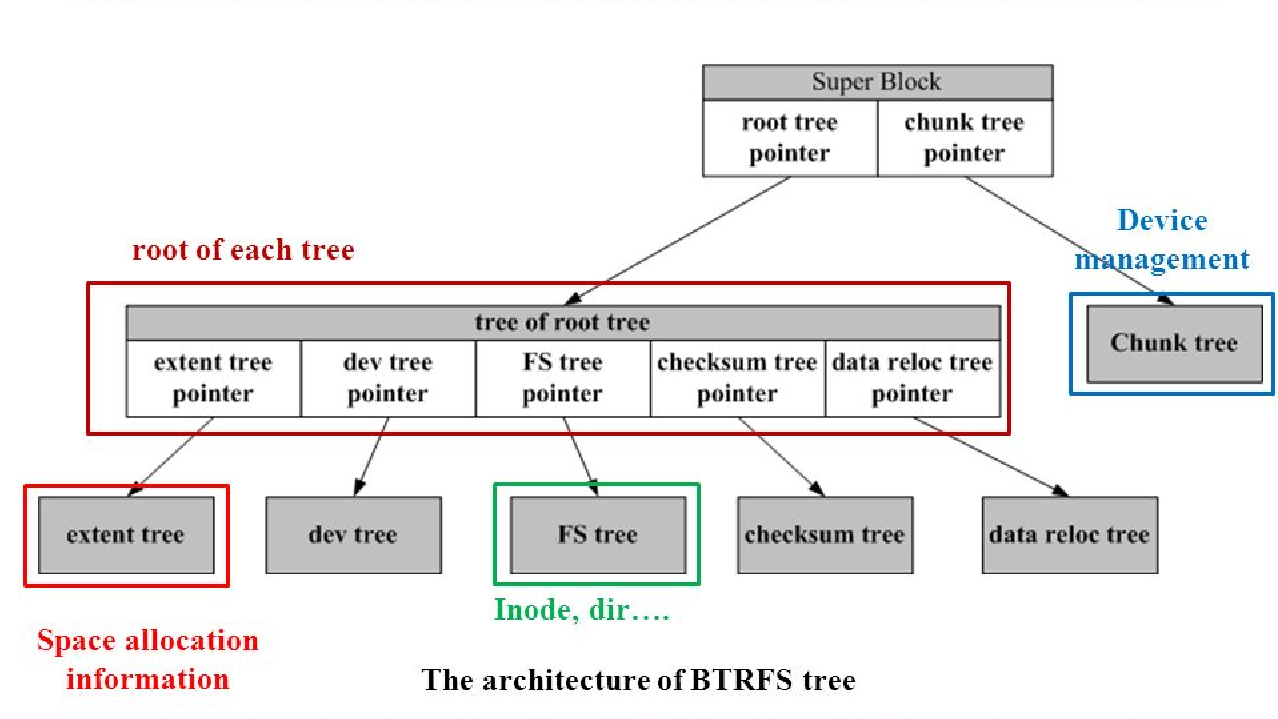
\includegraphics[width=.8\textwidth, height=.7\textheight]{img/btrfs-design.png}
	\end{figure}
}}

\frame{\frametitle{BtrFS - Copy on Write (CoW)}
	\only<1>{
		\centering
		Initiale Datei
		\begin{figure}
			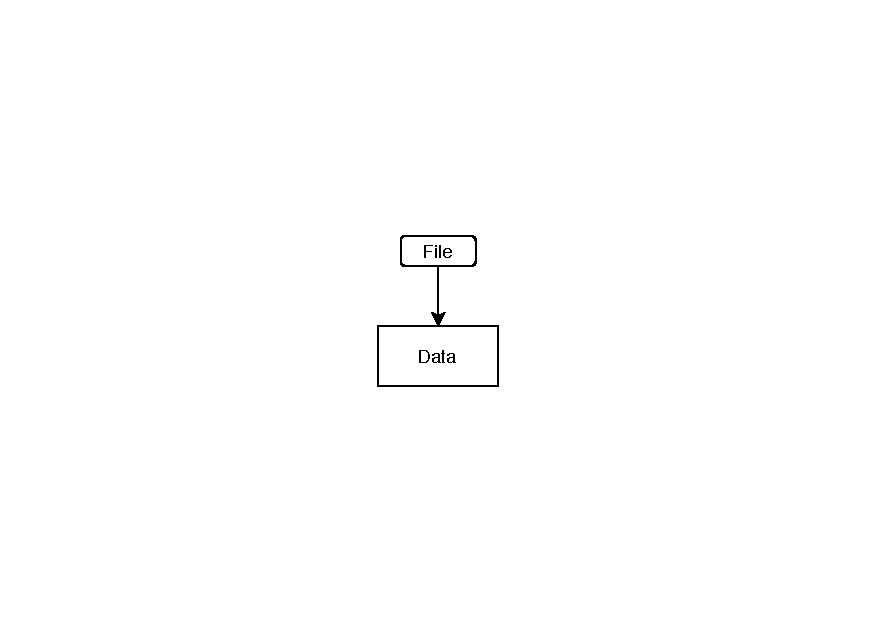
\includegraphics[width=.8\textwidth, height=.7\textheight]{img/cow1.pdf}
		\end{figure}}
	\only<2>{
		\begin{figure}
			\centering
			Initiale Datei und unveränderte Kopie
			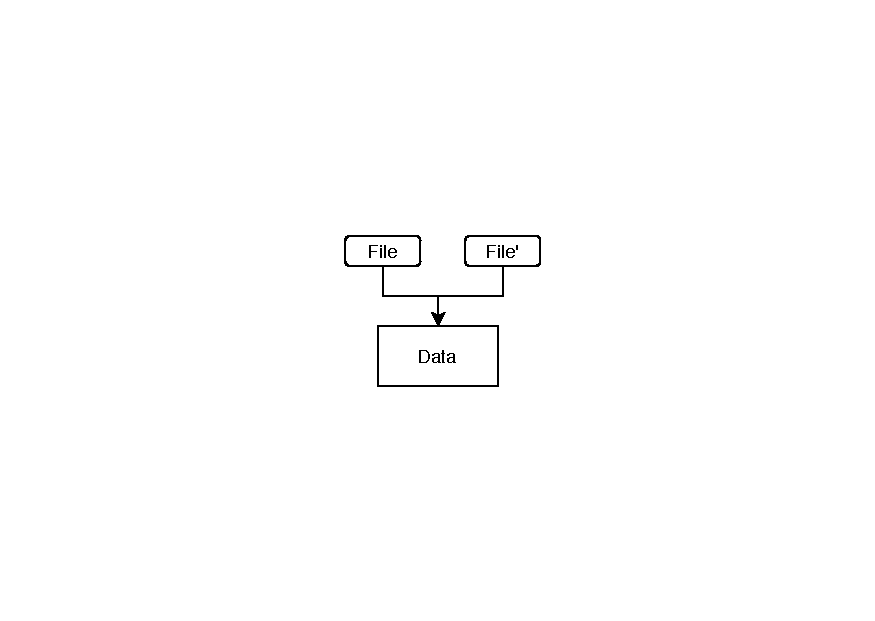
\includegraphics[width=.8\textwidth, height=.7\textheight]{img/cow2.pdf}
		\end{figure}}
	\only<3>{
		\begin{figure}
			\centering
			Kopie erfährt Anderungen 
			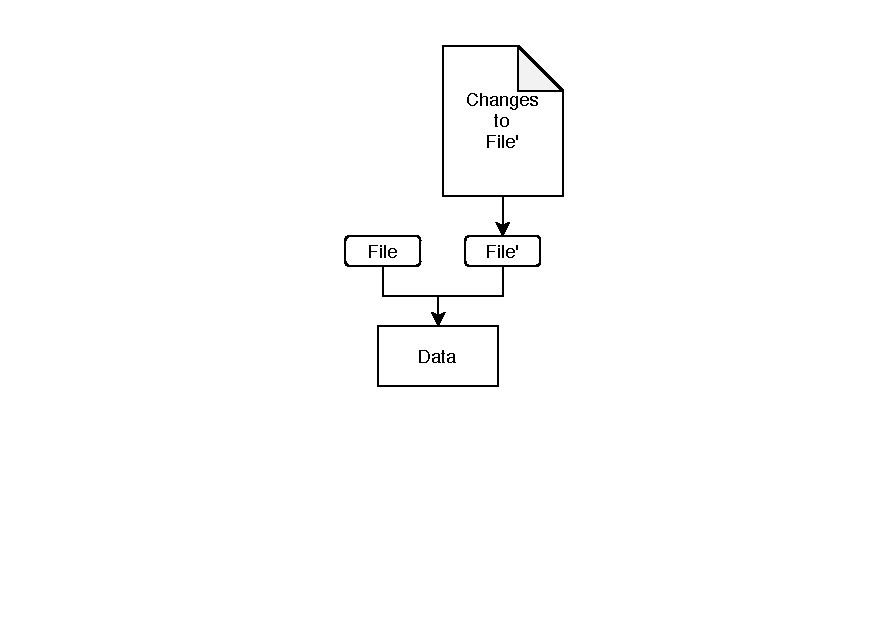
\includegraphics[width=.8\textwidth, height=.7\textheight]{img/cow3.pdf}
		\end{figure}}
	\only<4>{
		\begin{figure}
		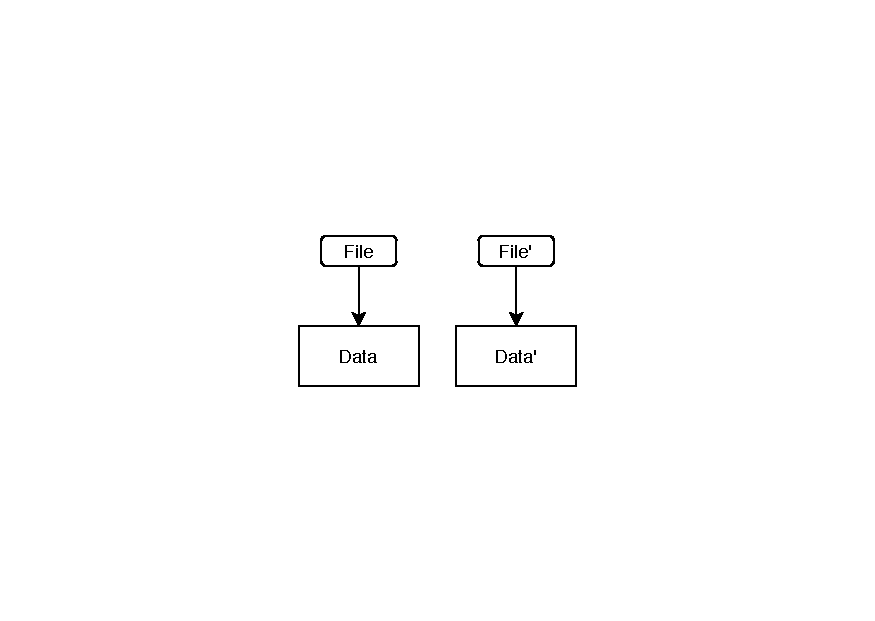
\includegraphics[width=.8\textwidth, height=.7\textheight]{img/cow4.pdf}
		\end{figure}}
}

\frame{\frametitle{BtrFS - Snapshots}
	\begin{figure}
		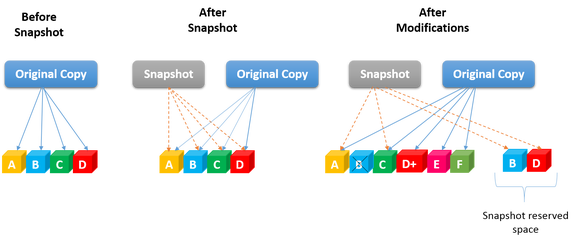
\includegraphics[width=.9\textwidth, height=.5\textheight]{img/btrfs-snapshot.png}
	\end{figure}
}

\frame{\frametitle{BtrFS - Data \& Metadata Checksum}
		\begin{figure}
		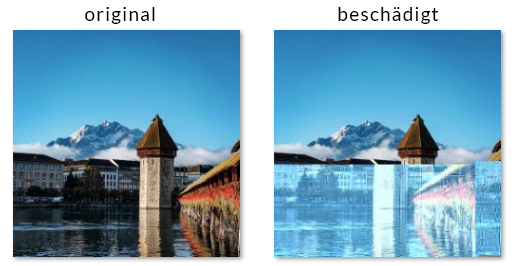
\includegraphics[width=.9\textwidth, height=.5\textheight]{img/bitrot.jpg}
	\end{figure}
}

\frame{\frametitle{BtrFS - Data \& Metadata Checksum}
	\begin{outline}
		\1 BtrFS generiert für alle Dateien und Metadaten eine Prüfumme
		\visible<2->{\1 Beim lesen eines defekten Extent, wird die Inkonsistenz der Prüfsummen festgestellt}
		\visible<3->{\2 mit Mirroring, korrekte Kopie wird gelesen und Defekt wird ersetzt
					 \2 ohne Mirroring, Extent wird verworfen und ein \emph{EIO} zurückgegeben}

		\visible<4->{\1 Mit \emph{btrfs scrub} für ganzes Dateisystem möglich}
	\end{outline}

	\visible<5->{
	\medskip
	dmesg \\
	\medskip
	\medskip
	\scriptsize
	[ 1120.891229] verify\_parent\_transid: 43 callbacks suppressed \\
	
	
	[ 1120.891243] parent transid verify failed on $16956989440$ wanted $13182$ found $12799$ \\
	
	
	[ 1124.851937] parent transid verify failed on $16585043968$ wanted $13145$ found $12357$ \\
	
	
	
	[ 1124.885429] btrfs read error corrected: ino 1 off 16977842176 (dev /dev/sdd sector 2921768)\\
	}
}

\frame{\frametitle{Redundant Array of Independent Disks (RAID)}
	\begin{outline}
		\1 Ermöglicht Organisation mehrerer Datenträger zu einem logischen Volume
		\1 Erlaubt effizientes redundantes Speichern
		\2 Rekonstruktion verlorener Daten bei Ausfall eines Dateiträgers
	\end{outline}
\visible<2->{Nachteile:
\begin{outline}
	\1 Fixe Plattengröße
	\1 Modifizierung erfordert Restriping
\end{outline}
}

}

\frame{\frametitle{BtrFS - RAID}
	\begin{outline}
		\1 RAID 0 (keine Parität) \&  1,5 (einfache Parität) \&  6 (mehrfache Parität)
		\visible<2->{\1 Keine einheitliche Plattengröße}
	\end{outline}
}

\frame[fragile=singleslide]{\frametitle{btrfs - RAID}
		\begin{outline}
			\1 RAID 0 (keine Parität) \&  1,5 (einfache Parität) \&  6 (mehrfache Parität)
			\1 Keine einheitliche Plattengröße
			\1 Dynamisches erweitern
		\end{outline}
	\verb|mkfs.btrfs -d <mode> -m <mode> <dev1> <dev2> ...| \\
	\verb|mount /dev/<disk x> /<mount point>| \\
	\verb|btrfs device add /dev/<disk y> /<mount point>|
}

\frame{\frametitle{BtrFS - RAID}
	\animategraphics[loop,controls,width=.95\linewidth]{2}{img/raid-ani1/btrfs-raid-ani1-}{0}{99}
}
\frame{\frametitle{BtrFS - RAID}
	\animategraphics[loop,controls,width=.95\linewidth]{2}{img/raid-ani2/btrfs-raid-ani2-}{0}{99}
}

%\begin{frame}
%	\transduration<0-99>{0}
%	\multiinclude[<+->][format=png, graphics={width=\textwidth}]{img/btrfs-raid-ani1}
%\end{frame}




\frame{\frametitle{BtrFS - Weitere Features}
	\begin{outline}
		\1 Snapshots, read-only Snapshots
		\1 BtrFS RAID (raid0, raid1, raid10, raid5 \& raid6)
		\visible<2->{
		\1 Komprimierung auf Filesystem Ebene
		\2 verfügbare Algorithmen: \emph{zlib, lzo \& zstd}
		\2 \emph{mount -o compress /dev/sdx}
		\2 \emph{btrfs filesystem defrag -r /path}
		\visible<3->{
		\1 Subvolumes
		\2 eigene interne Dateisystem roots
		\2 \emph{btrfs subvolume create \emph{name}}
		}
	}
	\end{outline}
}

\frame{\frametitle{BtrFS - Nachteile}
	\begin{outline}
		\1 $B^+$ Baum kann unbalanciert werden
		\2 manuelles rebalancieren
		\visible<2->{
		\1 CoW Mechanismus führt zu Inkonsistenzen OLTP Workload, fragwürdig für Datenbanken
	}
\visible<3->{
		\1 Berechnung des benötigten Speicherplatzes mit Snapshots
		\2 $\text{btrfs filesystem df /}$ anstatt $\text{df /}$
	}
	\end{outline}
}}

\section{F2FS}
\frame{\frametitle{F2FS}
\begin{itemize}
    \item Flash-Dateisystem von Samsung (veröffentlicht 2012)
    \item Entwickelt nur für Flash-Speicher (SD-Karte, SSDs, eMMC-Karten)
    \item Ziel: Optimierung der Performance und Lebenszeit von Flash-Speichern
    \item Entwickelt als Open-Source Projekt
    
    \item[ ] 
    \pause\item Verfolgt den Ansatz eine Log-structured File System (append-only logging)
    \item Arbeitet nicht auf ,,raw'' Flash-Zellen (Benötigt einen FTL)
    \item Viele Möglichkeiten zur Anpassung des Systems
    \item Verwendung von iNodes und Datenblöcken (Ähnlich zu UNIX)
    
    \item[ ] 
    \pause\item Verfügbar ab Linux Kernel 3.8  
    \item Verwendung in Huawei (2016), Galaxy Note 10, Google Nexus
\end{itemize}
}

\frame{\frametitle{F2FS - Flash-friendly on-disk Layout}
\begin{itemize}
    \item Einheiten: Blöcke, Segmente, Sektionen, Zonen
    \item Orientierung an FTL-Einheiten um Kosten zu Vermeiden
    \pause\item Metadaten: 
    \begin{itemize}
        \item Random Writes: Vorhalten in Arbeitsspeicher (Bei Checkpoints schreiben)
    \end{itemize}
    \pause\item Haupt-Speicherbereich:
    \begin{itemize}
        \item Aufgeteilt in Standardmäßig 4KB Blocks (Jeder Block ist Node- oder Data-Block)
        \item Node- und Data-Blocks liegen in verschiedenen Segmenten
    \end{itemize}
\end{itemize}
\visible<2->{
\begin{figure}[h]
	\centering
	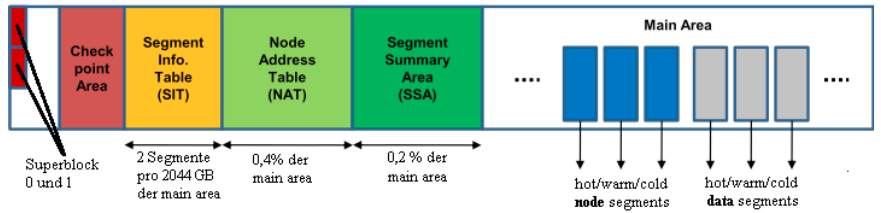
\includegraphics[width=\textwidth]{img/Figure_F2FS_ODL.png}
	\caption{on-disk Layout F2FS}
\end{figure}
}
}

\frame{\frametitle{F2FS - Besonderheiten I}
\begin{itemize}
    \item Multi-Head Logging
    \begin{itemize}
        \item Mehrere aktive Logsegmente parallel (Standard 6) 
        \item Parallele Verwendung durch Architektur möglich (multi-Streaming Interface)
        \item Unterscheidung der Daten in hot/warm/cold Schema (Update Frequenz)
    \end{itemize}
    \item[ ] 
    \pause\item Kosten-Effiziente Index Struktur
    \begin{itemize}
        \item Verwendung einer neuartigen Indexes: note adress table (NAT)
        \item Zur Vermeidung des ,,wandering tree'' Problems 
        \begin{itemize}
            \item Nur Update des direct Node Block und NAT
            \item Reduktion der Updates um Schreiboperationen zu sparen 
        \end{itemize}
    \end{itemize}
    
    
\end{itemize}
}

\frame{\frametitle{F2FS - Besonderheiten  II}
\begin{itemize}
    \item Adaptive logging
    \begin{itemize}
        \item Append-only Logging : Standardmäßig (random writes werden sequentiell)
        \item Threaded Logging : Verwendung bei hoher Auslastung (random writes)
    \end{itemize}
    \item[ ] 
    \pause
	\item Garbage Collection
    \begin{itemize}
        \item On-Demand: Wenn nicht genügend Speicherplatz verfügbar ist
        \begin{itemize}
            \item Greedy: Auswahl des Opfersegments mit wenigsten gültigen Blöcken
        \end{itemize}
        \item Background: Bei geringer Auslastung des Systems von Kernel ausgeführt
        \begin{itemize}
            \item Kosten-Effizient: Auswahl durch Segment-Alter und Anzahl gültiger Blöcke
        \end{itemize}
    \end{itemize}
\end{itemize}
}

\frame{\frametitle{F2FS - Bewertung}

\begin{itemize}
    \item Vorteile
    \begin{itemize}
        \item Optimierung der Zusammenarbeit von FTL und Dateisystem
        \item Vermeidung des Wandering Tree Problems
        \item Anpassung des Dateisystems an System-Status
        \item Hohe Anzahl an Parametern um Dateisystem anzupassen
    \end{itemize}
    
    \pause\item Nachteile
    \begin{itemize}
        \item Nur für Flash-Speicher (mit einem FTL)
        \item FTL Qualität wichtiges Kriterium 
        \item Initialer hoher belegter Speicherplatz durch Metadaten
        \item Hohe CPU-Belastung beim Schreiben von Dateien
    \end{itemize}
\end{itemize}
	
}

\section{Benchmarks}
\frame{\frametitle{Benchmarks - F2FS Results}
	\begin{figure}[h]
		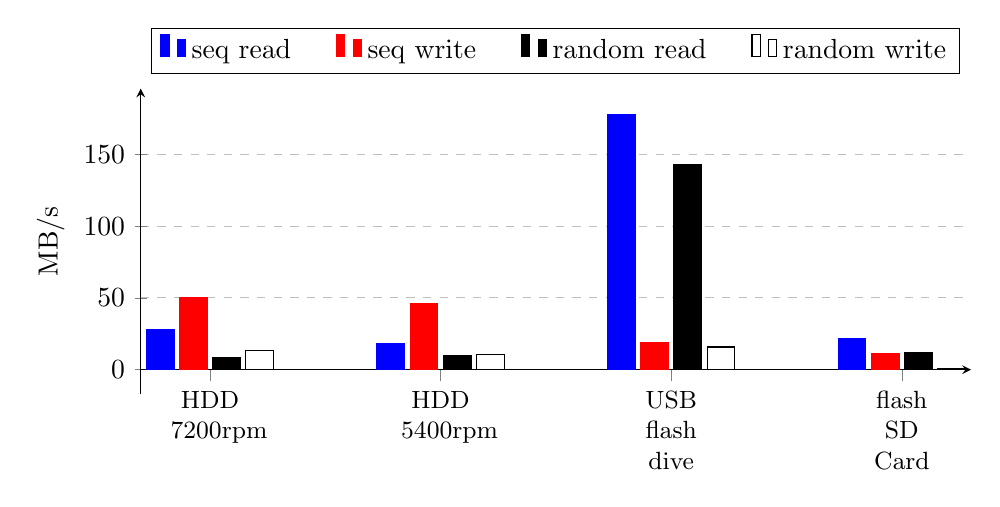
\begin{tikzpicture}
		\begin{axis}[
		width=\textwidth,
		height=0.45\textwidth,
		axis x line=center,
		axis y line=left,
		x label style={at={(axis description cs:0.5,-0.1)},anchor=north},
		ylabel={MB/s},
		symbolic x coords={HDD 7200rpm, HDD 5400rpm, USB flash dive,flash SD Card},
		x tick label style={font=\small,text width=1cm,align=center},
		xtick=data,
		enlargelimits=true,
		legend style={
			at={(0.5,1.2)},
			anchor=north,
			legend columns=-1,
			/tikz/every even column/.append style={column sep=0.5cm}
		},	
		ymajorgrids=true,
		grid style=dashed,
		ybar
		]
		\addplot[color=blue,fill]
		coordinates {(HDD 7200rpm, 27.7)(HDD 5400rpm, 18.3)(USB flash dive, 178)(flash SD Card,21.9)};
		\addplot[color=red,fill]
		coordinates {(HDD 7200rpm, 50)(HDD 5400rpm, 46.1)(USB flash dive, 18.6)(flash SD Card,10.9)};
		\addplot[color=black,fill]
		coordinates {(HDD 7200rpm, 8.7)(HDD 5400rpm, 9.7)(USB flash dive, 143)(flash SD Card, 11.6)};
		\addplot[color=black]
		coordinates {(HDD 7200rpm, 13.4)(HDD 5400rpm, 10.3)(USB flash dive, 15.8)(flash SD Card, 0.9)};
		\legend{seq read, seq write, random read, random write}
		\end{axis}
		\end{tikzpicture}
		\caption{F2FS raw performance}
	\end{figure}
}

\frame{\frametitle{Benchmarks - BtrFS Results}
\begin{figure}[h]
	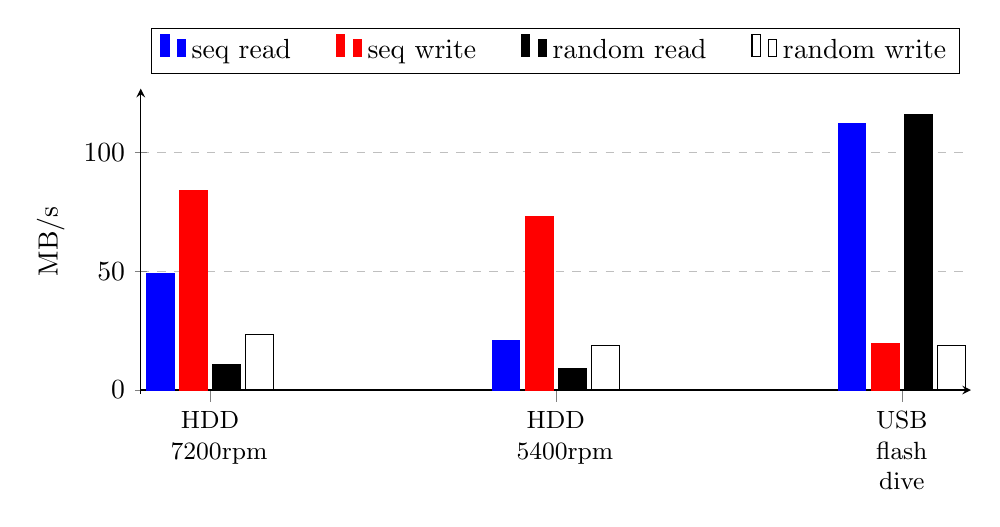
\begin{tikzpicture}
	\begin{axis}[
	width=\textwidth,
	height=0.45\textwidth,
	axis x line=center,
	axis y line=left,
	x label style={at={(axis description cs:0.5,-0.1)},anchor=north},
	ylabel={MB/s},
	symbolic x coords={HDD 7200rpm,HDD 5400rpm,USB flash dive},
	x tick label style={font=\small,text width=1cm,align=center},
	xtick=data,
	enlargelimits=true,
	legend style={
		at={(0.5,1.2)},
		anchor=north,
		legend columns=-1,
		/tikz/every even column/.append style={column sep=0.5cm}
	},	
	ymajorgrids=true,
	grid style=dashed,
	ybar
	]
	\addplot[color=blue,fill]
	coordinates {(HDD 7200rpm, 49)(HDD 5400rpm,20.6)(USB flash dive,112)};
	\addplot[color=red,fill]
	coordinates {(HDD 7200rpm, 84)(HDD 5400rpm, 73.1)(USB flash dive, 19.5)};
	\addplot[color=black,fill]
	coordinates {(HDD 7200rpm, 10.5)(HDD 5400rpm, 9.1)(USB flash dive, 116)};
	\addplot[color=black,]
	coordinates {(HDD 7200rpm, 23.5)(HDD 5400rpm, 18.7)(USB flash dive, 18.6)};
	\legend{seq read, seq write, random read, random write}
	\end{axis}
	\end{tikzpicture}
	\caption{BtrFS raw performance}
\end{figure}
}


\frame{\frametitle{Benchmarks - Btrfs Results}
	\begin{figure}[h]
		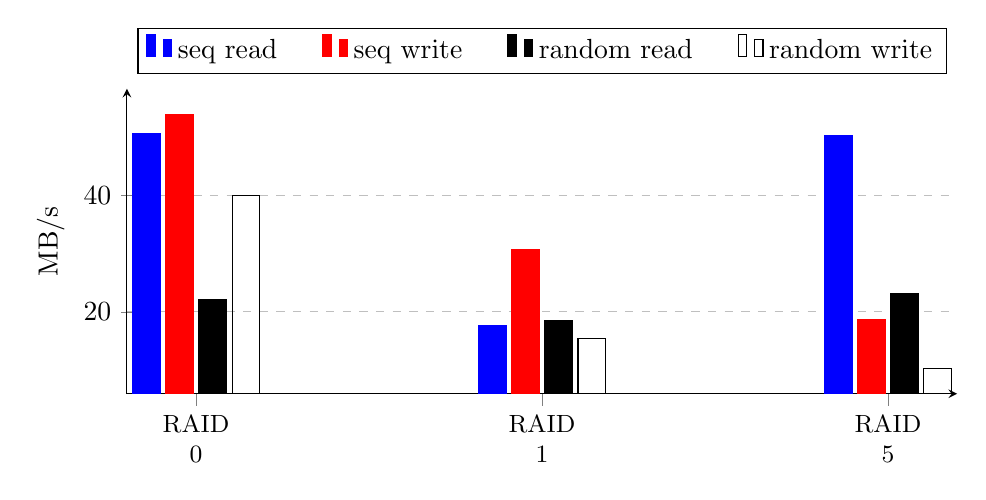
\begin{tikzpicture}
		\begin{axis}[
		width=\textwidth,
		height=0.45\textwidth,
		axis x line=center,
		axis y line=left,
		x label style={at={(axis description cs:0.5,-0.1)},anchor=north},
		ylabel={MB/s},
		symbolic x coords={RAID 0, RAID 1, RAID 5},
		x tick label style={font=\small,text width=1cm,align=center},
		xtick=data,
		enlargelimits=true,
		legend style={
			at={(0.5,1.2)},
			anchor=north,
			legend columns=-1,
			/tikz/every even column/.append style={column sep=0.5cm}
		},	
		ymajorgrids=true,
		grid style=dashed,
		ybar
		]
		\addplot[color=blue,fill]
		coordinates {(RAID 0, 50.6)(RAID 1,17.6 )(RAID 5,50.4)};
		\addplot[color=red,fill]
		coordinates {(RAID 0, 54 )(RAID 1, 30.8)(RAID 5, 18.7)};
		\addplot[color=black,fill]
		coordinates {(RAID 0, 22.2)(RAID 1, 18.6)(RAID 5, 23.2)};
		\addplot[color=black]
		coordinates {(RAID 0, 40)(RAID 1, 15.5)(RAID 5, 10.3)};
		\legend{seq read, seq write, random read, random write}
		\end{axis}
		\end{tikzpicture}
		\caption{BtrFS RAID performance}
	\end{figure}
}
\frame{\frametitle{Benchmarks - BtrFS vs. F2Fs}
	\begin{figure}[h]
		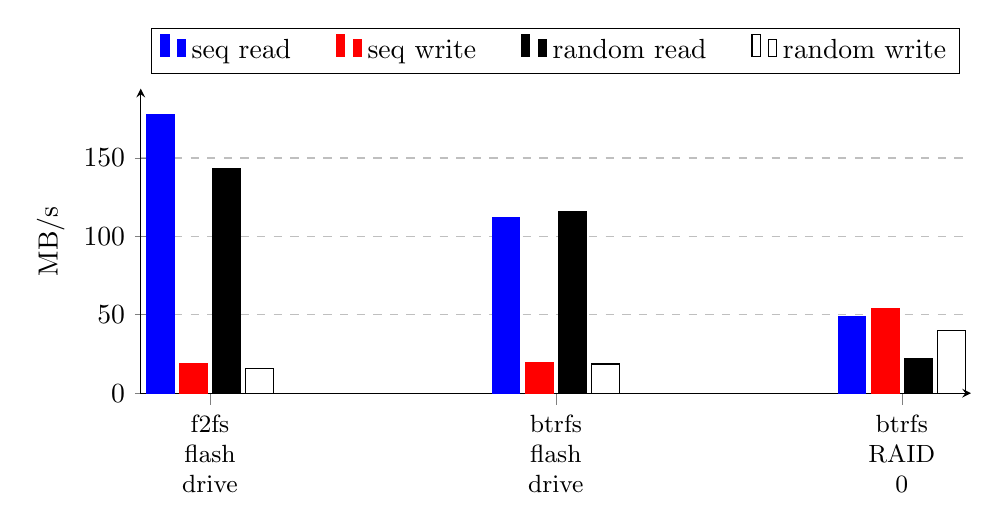
\begin{tikzpicture}
		\begin{axis}[
		width=\textwidth,
		height=0.45\textwidth,
		axis x line=center,
		axis y line=left,
		x label style={at={(axis description cs:0.5,-0.1)},anchor=north},
		ylabel={MB/s},
		symbolic x coords={f2fs flash drive,btrfs flash drive,btrfs RAID 0},
		x tick label style={font=\small,text width=1cm,align=center},
		xtick=data,
		enlargelimits=true,
		legend style={
			at={(0.5,1.2)},
			anchor=north,
			legend columns=-1,
			/tikz/every even column/.append style={column sep=0.5cm}
		},	
		ymajorgrids=true,
		grid style=dashed,
		ybar
		]
		\addplot[color=blue,fill]
		coordinates {(f2fs flash drive, 178)(btrfs flash drive,112)(btrfs RAID 0, 48.6)};
		\addplot[color=red,fill]
		coordinates {(f2fs flash drive, 18.6)(btrfs flash drive, 19.5)(btrfs RAID 0, 54)};
		\addplot[color=black,fill]
		coordinates {(f2fs flash drive, 143)(btrfs flash drive, 116)(btrfs RAID 0, 22.2)};
		\addplot[color=black,]
		coordinates {(f2fs flash drive, 15.8)(btrfs flash drive, 18.6)(btrfs RAID 0,40)};
		\legend{seq read, seq write, random read, random write}
		\end{axis}
		\end{tikzpicture}
		\caption{F2FS vs. BtrFS vs. BtrFS RAID0}
	\end{figure}
}

\frame{\frametitle{Literatur}
\printbibliography[]
}

\end{document}